\documentclass{memoir}
\usepackage[utf8]{inputenc}
\usepackage{import}
\usepackage[english]{babel}
% \usepackage{standalone}
\usepackage{geometry}
 \geometry{
 a4paper,
 total={170mm,257mm},
 left=20mm,
 top=20mm,
 }
\usepackage{graphicx}
\usepackage{amsfonts}
\usepackage{url}
\usepackage[final]{pdfpages}

\usepackage{color}                    				%Creates coloured text and background
\usepackage[colorlinks=true,
		     allcolors=black]{hyperref} 

%  \usepackage{titling}

\title{Adaptation Approach}
\author{Christian Bauer}
% \date{November 2022}
 
 \usepackage{fancyhdr}

\begin{document}

  \maketitle

  \tableofcontents
  \listoffigures
  

  \section*{Abstract}

  \chapter*{Publications of the Thesis}

    \section*{Big Data Pipeline Scheduling and Adaptation on the Computing Continuum}

    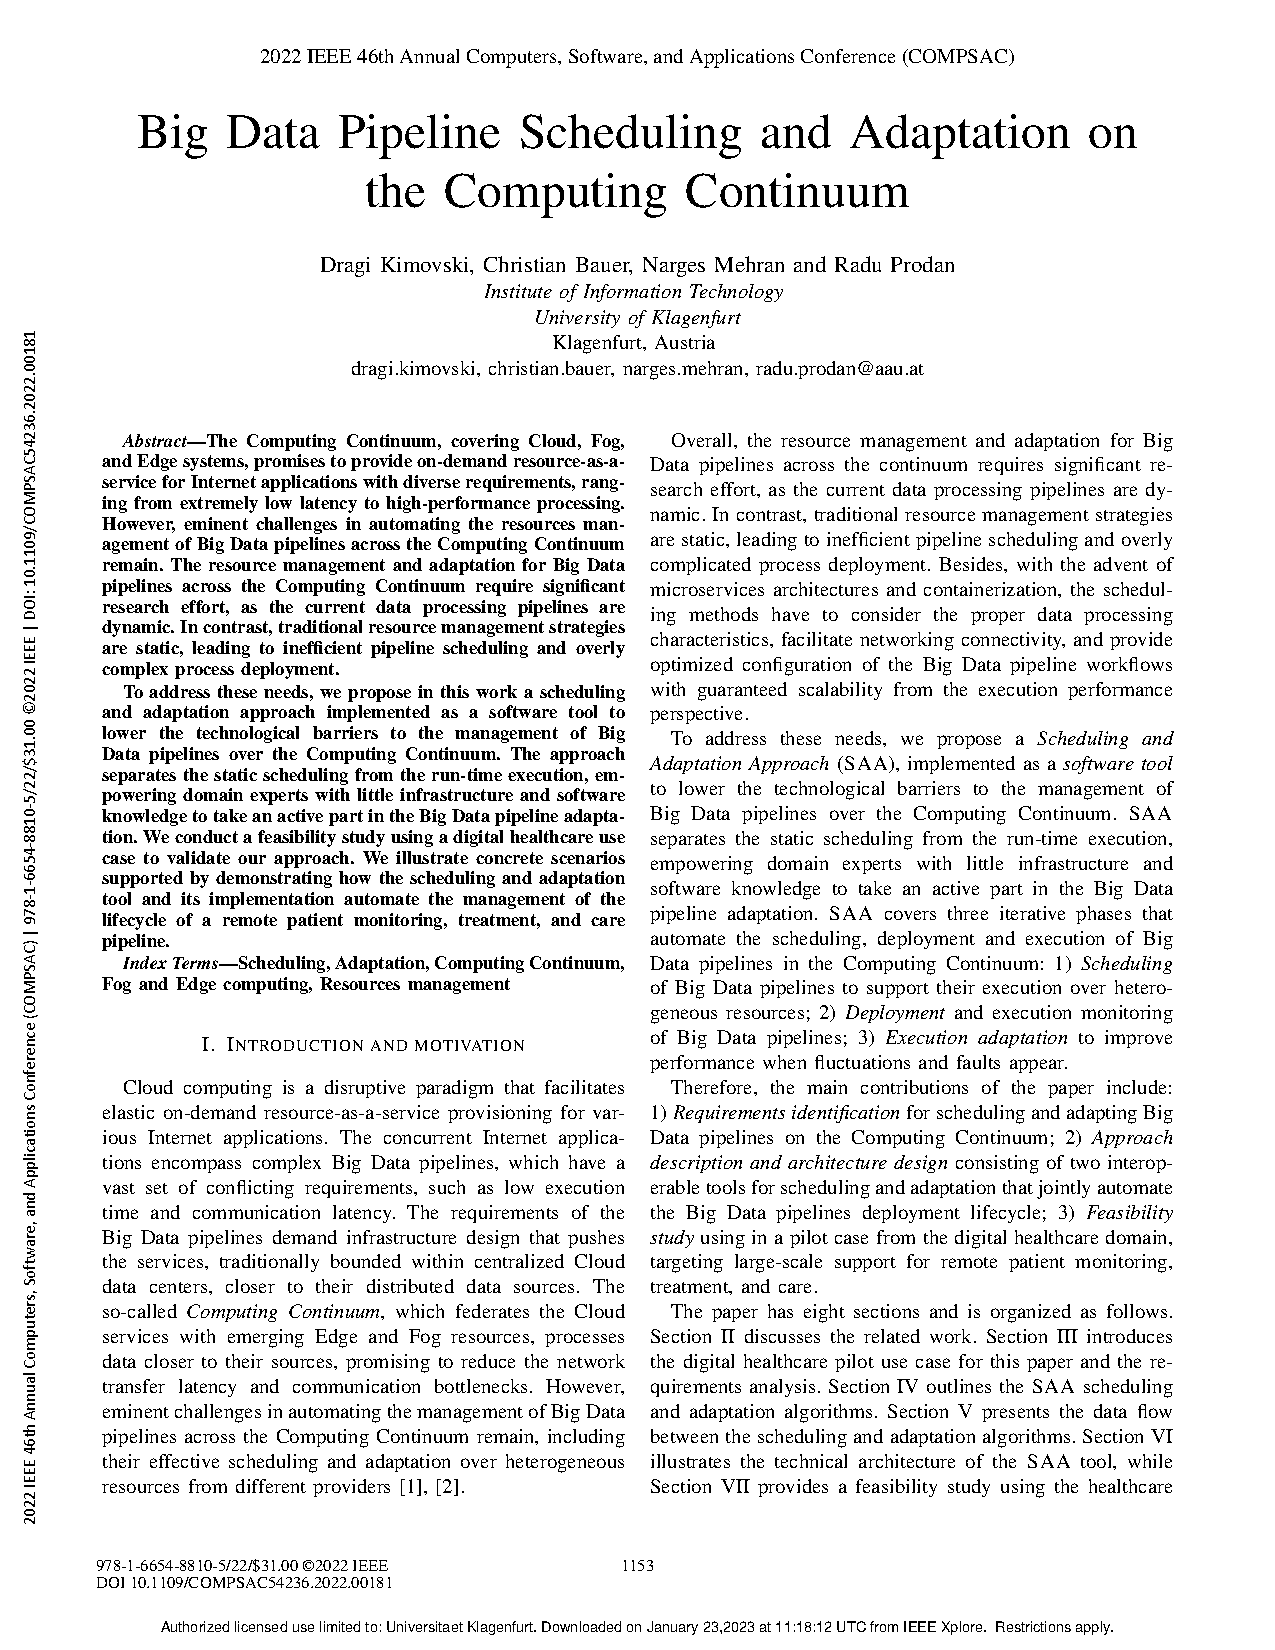
\includepdf[pages=-,pagecommand={},width=\textwidth]{papers/Big_Data_Pipeline_Scheduling_and_Adaptation_on_the_Computing.pdf}
    

  \import{./chapters/1_introduction}{introduction.tex}

  \import{chapters/2_sota_background}{background.tex}
  \import{chapters/2_sota_background}{state_of_the_art.tex}

  \import{chapters/3_model}{model.tex}

  \import{chapters/4_architecture_and_implementation}{architecture_and_implementation.tex}
  
  \import{chapters/5_evaluation_and_results}{evaluation_and_results.tex}

  \import{chapters/6_conclusions_and_future_work}{conclusions_and_future_work.tex}



  \bibliographystyle{ieeetr}
  \bibliography{references}



\end{document}

